\section{BACKGROUND}
\subsection{Game Theory}
\label{subsec: game_theory}
Game theory is a wide area of research which is used in various areas such as economics, computer architecture,  computer security and robotics. Two main aspects of a scenario modelled in game theory are the well defined utility and the information, each player has \cite{OR94}. For a game theory problem, there has to be more than one party involved. 
\par In a broad sense, games theory categorizes four kinds of games namely strategic games, extensive games with perfect information, extensive games without perfect information and coaliational games.

\paragraph{Strategic Games}\cite{OR94}
In a strategic game we have a set $P$ of players and each player $P_i$ has a non empty set of actions $A_i$. Each $P_i$ has a preference relation $\geq_i$ defined in $A_1 \times A_2 \times \cdots A_n$ which denotes how a player is affected from different action combinations. An action is denoted $(a_1,a_2, \cdots , a_n)$. As a short notation to compact the action combination of the players other than $P_i$ we use $a_{-i}$. The action combination $(a_1,a_2, \cdots , a_n)$ can also written as $(a_{-i},a_i)$ when we want to explicitly differentiate between player $P_i$'s actions and actions of the other players. This notation can be extended to denote the action combinations of player sets. For a set $st$, $(a_{st},a_{[n]-st})$
denotes the corresponding actions are categorized w.r.t the player set. 
\newline A Pay off function is defined for a special case where the preference relation is a total order. 
\paragraph{Extensive games with perfect information}\cite{OR94}
These kind of games have a set $P$ of players and a set of sequences (finite or infinite) $H$ which stand for the history of actions of a game. A member $h \in H$ is called terminal (history towards end of a game) if $h$ is infinite or not a prefix of any other member in $H$. We use Z to denote the set of all terminal sequences in $H$. A preference relation (similar for strategic game) is defined for these terminal sequences. For all the non terminal sequences in $H$ a function $Turn: H \setminus Z \rightarrow P $  specifies the player who has the next move. A player can choose between a set of actions depending on his history $h$. Here perfect information refers to the fact that at any point of the game all the players have history information.

\paragraph{Extensive games without perfect information}\cite{OR94}
In contrast to extensive games with perfect information, this type of games have a probability distribution for the set of actions to perform given a history $h$. In addition to the probability, there are information partitions defined for each player. All the history sequences where the resulting action set is similar are categorized into same partition. When a player does not know his exact history but knows all the possibilities for history and his action set can short list the possible history values according to information partitions.

\paragraph{Coalitional games}

Coalitional games are described for the completeness. Coalition games have a set $P$ of players and it has a value function $V : \mathbb{P} P \setminus \phi \rightarrow \mathbb{R}$ to define the pay off value obtained for each coalition.

\paragraph{Nash Equilibrium}\cite{OR94}
Nash Equilibrium is a state of a game ending in which no player has a regret on the strategy he used when he cannot control the strategies of other players. We define a Nash equilibrium for a strategic game as follows. \newline

\begin{definition}
	For a  strategic game of player set $P$ and action set $A_1\times A_2 \times \cdots \times A_n$ and preference relation $\geq$ a nash equilibrium is defined as an action combination $a^{*} \in $ such that, \\
$	\forall P_i \in P$ \\
$(a_{-i}^{*},a_i^{*}) \geq_i (a_{-i}^{*},a_i) \forall a_i \in A_i$
\end{definition}
It is not always the case that, a nash equilibrium according to above definition exists. However, for any strategic game, a mixed strategy Nash equilibrium exists. Nash Equilibrium for other forms of games also have the same concept of best response. We will not discuss all the definitions here, and we will refer to specific Nash Equilibrium definitions in section \ref{sec: verification_algo}.

In computer science research, the most important aspect we look in game theory is, computation and verification of Nash equilibria. The computation complexity is highly dependant with the number of strategies. Calculating Nash equilibrium in strategic games is PPAD complete. \cite{DGP09},\cite{CD06}. \newline
Extensive form games are widely used to model actual games in real life where the players take turns. There are some applications that can be regarded as games and can be represented by non of the above game categories. For example, processes/protocols can be defined as finite state mechanisms. However, the closest representation of the above mentioned representations is extensive form. This representation itself is not very efficient. 

%\par
%Multiparty computation protocols can also be analyzed using game theory. \cite{ADGH06} and \cite{ADGH06} analyze how the Shamir secret sharing scheme can be modified to be resilient to coaliation attacks.
%In \cite{ADGH06} a general strategy for any player. The $m$ out of $n$ secret sharing is augmented with a mediator for the following game. Mediator has a random variable $c^t\in \{0,1\} $ for each time step such that $Pr(c^{t}=\alpha)$ and $h^{t}=fc^{t} + g^{t}$ if $c^{t}=1$ $h^{t}(0)=f(0)$ which is the value of the secret. otherwise $f(0)$ cannot be calculated since $g^{t}(0)$ would always be chosen to be $0$. If any player can calculate $h^{t}(0)$ at some iteration when $c^{t}=1$ then he would know the secret. The paper analyzes how the players can know the secret by acting as coaliators. They find an upper bound to $\alpha$ such that the game is $k$-resilient. Paper suggests some changes to the mediator's protocol such that expected running time is reduced.Can we verify k-resilience by using model checking?  We can verify k-resilience for specific $n$.Utility functions had to be defined to fit the conditions mentioned in the paper. 
%
%%%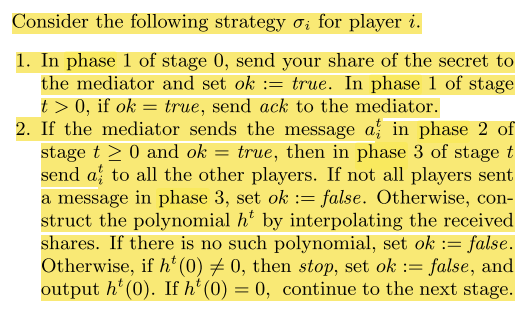
\includegraphics{strategy}
%
%\cite{CJM98} implements a natural deduction based model checker to identify attacks on security protocols. \cite{TL10} describes a PAT approach. This introduces a new language called "Seve" to specify security protocols and also introduces a translator to translate from "Seve" to RTS. to RTS.  
%
%Try model bitcoin.Look at contract signing.Do some review in PRISM papers.
%
%probabilistic trusted 3rd party.
